\documentclass{beamer}

\usetheme{Boadilla}
\useoutertheme{split}


\usepackage{amsmath,latexsym,amsthm,amssymb,amsfonts,amscd,stmaryrd,textcomp} % math. symbols

% Corporate design stuff
\usepackage[absolute]{textpos}
\usepackage{blindtext}
\usepackage{helvet}
\usepackage{color}




%---- language -------%
\usepackage[english]{babel} % English spelling
\usepackage[backend=bibtex,style=alphabetic,citestyle=alphabetic]{biblatex}
\addbibresource{bib.bib} %Imports bibliography file

% define commands with auto-spacing command \xspace
\usepackage{xspace} 
% comma placement
\usepackage{icomma} 


\usepackage[perpage]{footmisc}



\usepackage{listings}
\usepackage{float}
\usepackage{graphicx}
\usepackage{caption}
\usepackage{subcaption}

\usepackage{appendix}
\usepackage{tikz}
\usepackage{xcolor}

\usepackage{algorithm}
\usepackage[ruled,vlined, algo2e, noend]{algorithm2e}
\usepackage{bytefield}
\usepackage{multicol}
\usepackage{multirow}

\usepackage[T1]{fontenc}  

\usetikzlibrary{arrows,calc,shapes,shadows,decorations.pathmorphing,decorations.pathreplacing,automata,shapes.multipart,positioning}

\usepackage[final]{pdfpages}
\usepackage{newclude}
\usepackage{tcolorbox}
\usepackage{xcolor}
\usepackage{pagecolor}
\usepackage{url}
\usepackage{datetime}
\usepackage{enotez}
\usepackage[absolute]{textpos}
\usepackage{mathtools}
%Put your commands here!

\newcommand{\sep}{\ensuremath{~\mid~}}
\newcommand{\xor}{\mathbin{\oplus}}
\newcommand{\bow}{\mathbin{\bowtie}}



\newcommand{\colorbitbox}[3]{%
	\rlap{\bitbox{#2}{\color{#1}\rule{\width}{\height}}}%
	\bitbox{#2}{#3}}
\definecolor{lightcyan}{rgb}{0.84,1,1}
\definecolor{lightgreen}{rgb}{0.64,1,0.71}
\definecolor{lightred}{rgb}{1,0.7,0.71}

%\renewcommand{\thesection}{\Roman{section}} 
%\renewcommand{\thesubsection}{\thesection.\Roman{subsection}}
%
%\titleformat{\section}{\normalfont\Large\bfseries}{}{0em}{(\thesection) #1\ }

\tikzset{>=latex} % for LaTeX arrow head
\usepackage{xcolor}
\colorlet{myred}{red!80!black}
\colorlet{myblue}{blue!80!black}
\colorlet{mygreen}{green!60!black}
\colorlet{myorange}{orange!70!red!60!black}
\colorlet{mydarkred}{red!30!black}
\colorlet{mydarkblue}{blue!40!black}
\colorlet{mydarkgreen}{green!30!black}
\tikzstyle{node}=[thick,circle,draw=myblue,minimum size=15]
\tikzstyle{node in}=[node,green!20!black,draw=mygreen!30!black,fill=mygreen!25]
\tikzstyle{node latent}=[node,blue!20!black,draw=myblue!30!black,fill=myblue!20]
\tikzstyle{node convol}=[node,orange!20!black,draw=myorange!30!black,fill=myorange!20]
\tikzstyle{node out}=[node,red!20!black,draw=myred!30!black,fill=myred!20]
\tikzstyle{connect}=[thick,mydarkblue] %,line cap=round
\tikzstyle{connect arrow}=[-{Latex[length=4,width=3.5]},thick,black,shorten <=0.2,shorten >=0.1]
\tikzset{ % node styles, numbered for easy mapping with \nstyle
	node 1/.style={node in},
	node 2/.style={node convol},
	node 3/.style={node out},
	node 4/.style={node latent},
}
\tikzstyle{flow} = [rectangle, draw, text centered, rounded corners]
\tikzstyle{connector} = [draw, -latex']




\title{Convolutional autoencoder for compression of neural data}
\subtitle{CNN for signal compression}
\author{Philip Kroll}
\institute{RWTH Aachen}
\newdate{date}{15}{02}{2023}
\date{\displaydate{date}}
%\date{\today}

\mode<presentation>{}

\begin{document}

\begin{frame}
    \titlepage
\end{frame}

\begin{frame}{Background}
	\only<1->{Goal : Investigation of pathological firing in pain receptors}
		\begin{itemize}
			\item<2-> Thin electrode is injected to record action potentials
			\item<3-> Sort those action potentials to individual nerves fibres
		\end{itemize}
		\only<4->{\begin{figure}
				\centering
				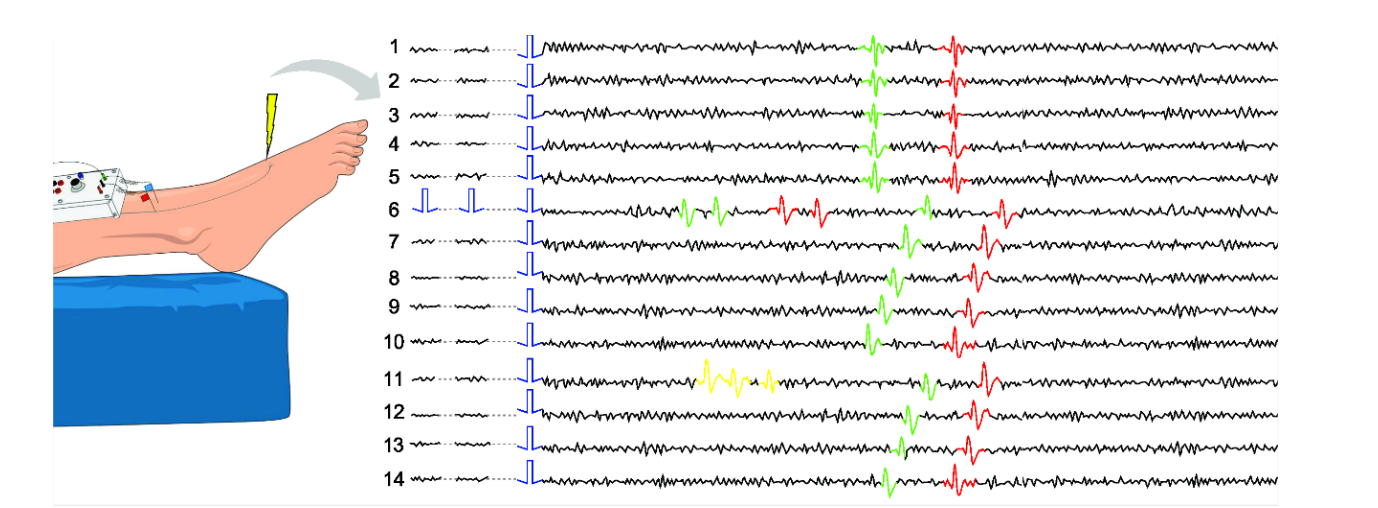
\includegraphics[width=\textwidth]{./Images/marking_method_1.png}
				\caption*{Example of the marking method}
		\end{figure}}
\end{frame}

\begin{frame}{Why signal compression?}
	\only<0-4>{\begin{figure}
			\centering
			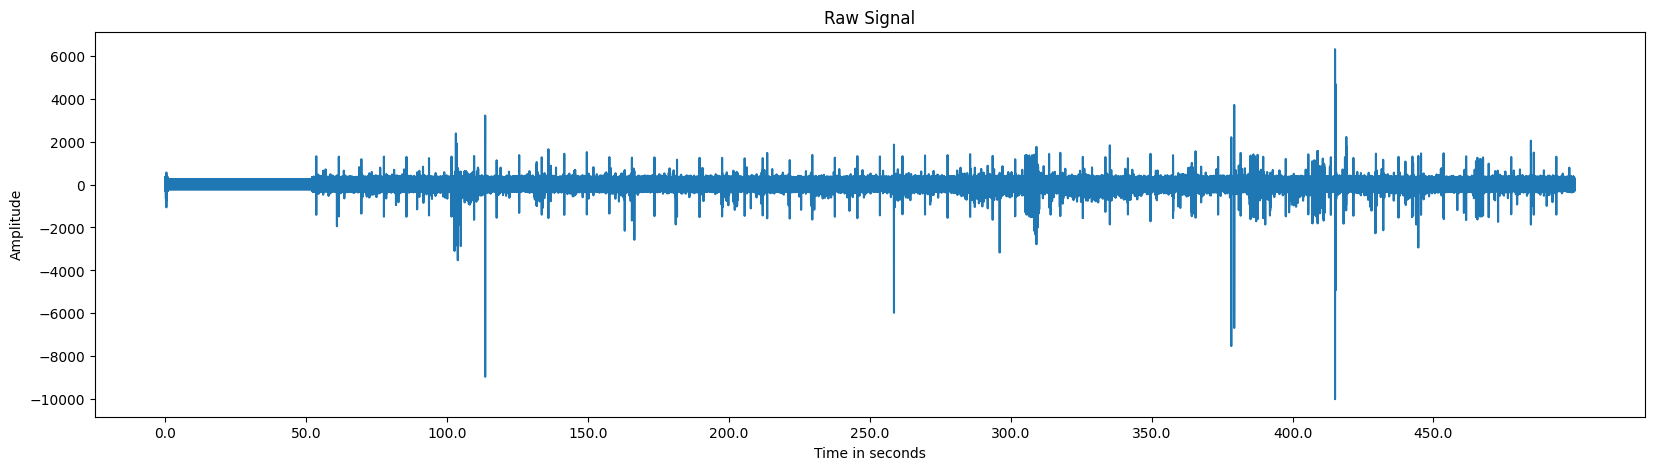
\includegraphics[width=\textwidth]{./../../Images/signal_segment.png}
	\end{figure}}
	\only<5>{\begin{figure}
		\centering
		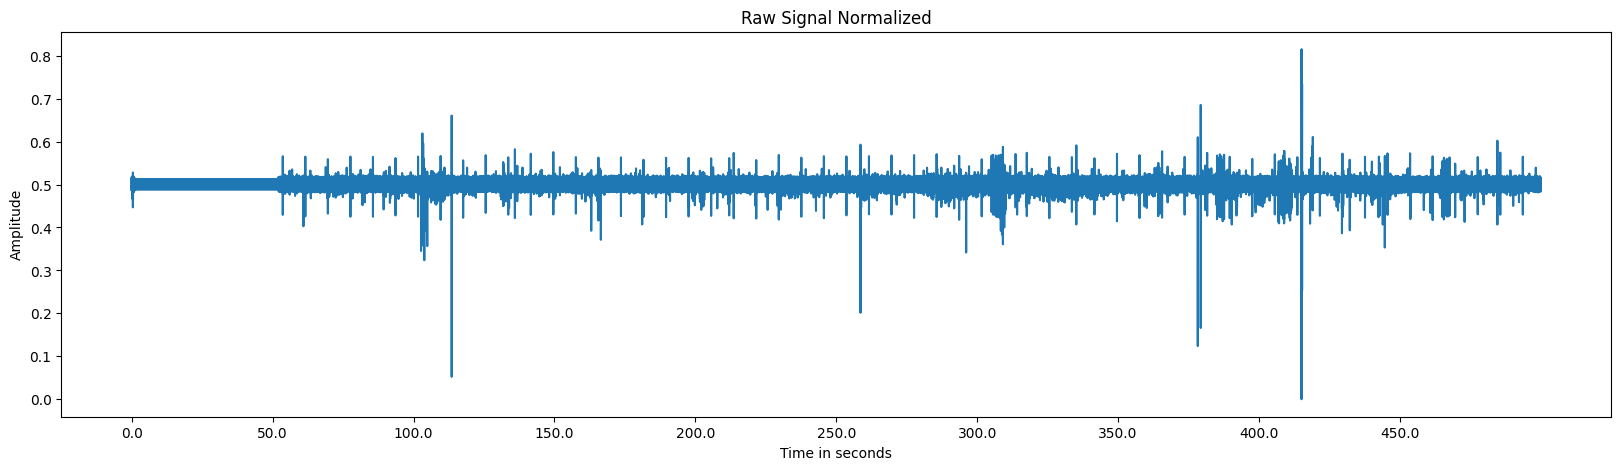
\includegraphics[width=\textwidth]{./../../Images/signal_segment_normalized.png}
\end{figure}}
	\begin{itemize}
		\item<1-> Low signal-to-noise ratio
		\item<1-> High variability in spike shapes
		\item<2-> Problems: {\begin{itemize}
				\item Identifying the spikes
				\item Sorting spikes to individual nerve fibres
		\end{itemize}}
		\item<3-> Standard Sorting \& Clustering Algorithms can not be used
	\end{itemize}
	\centering{\only<4->{$\Rightarrow$ We need to process the data such that it is usable}}
	\begin{itemize}
		\item<5-> For the following: Normalize Signal to range $[0,1]$
	\end{itemize}
\end{frame}

\begin{frame}{How does the compression work?}
    \begin{itemize}
    	\item<1-> Machine Learning \only<2->{ Neural Network (Autoencoder)}
    \end{itemize}


	\begin{minipage}[t]{0.6\textwidth}
			\only<3->{\begin{figure}
				\centering
				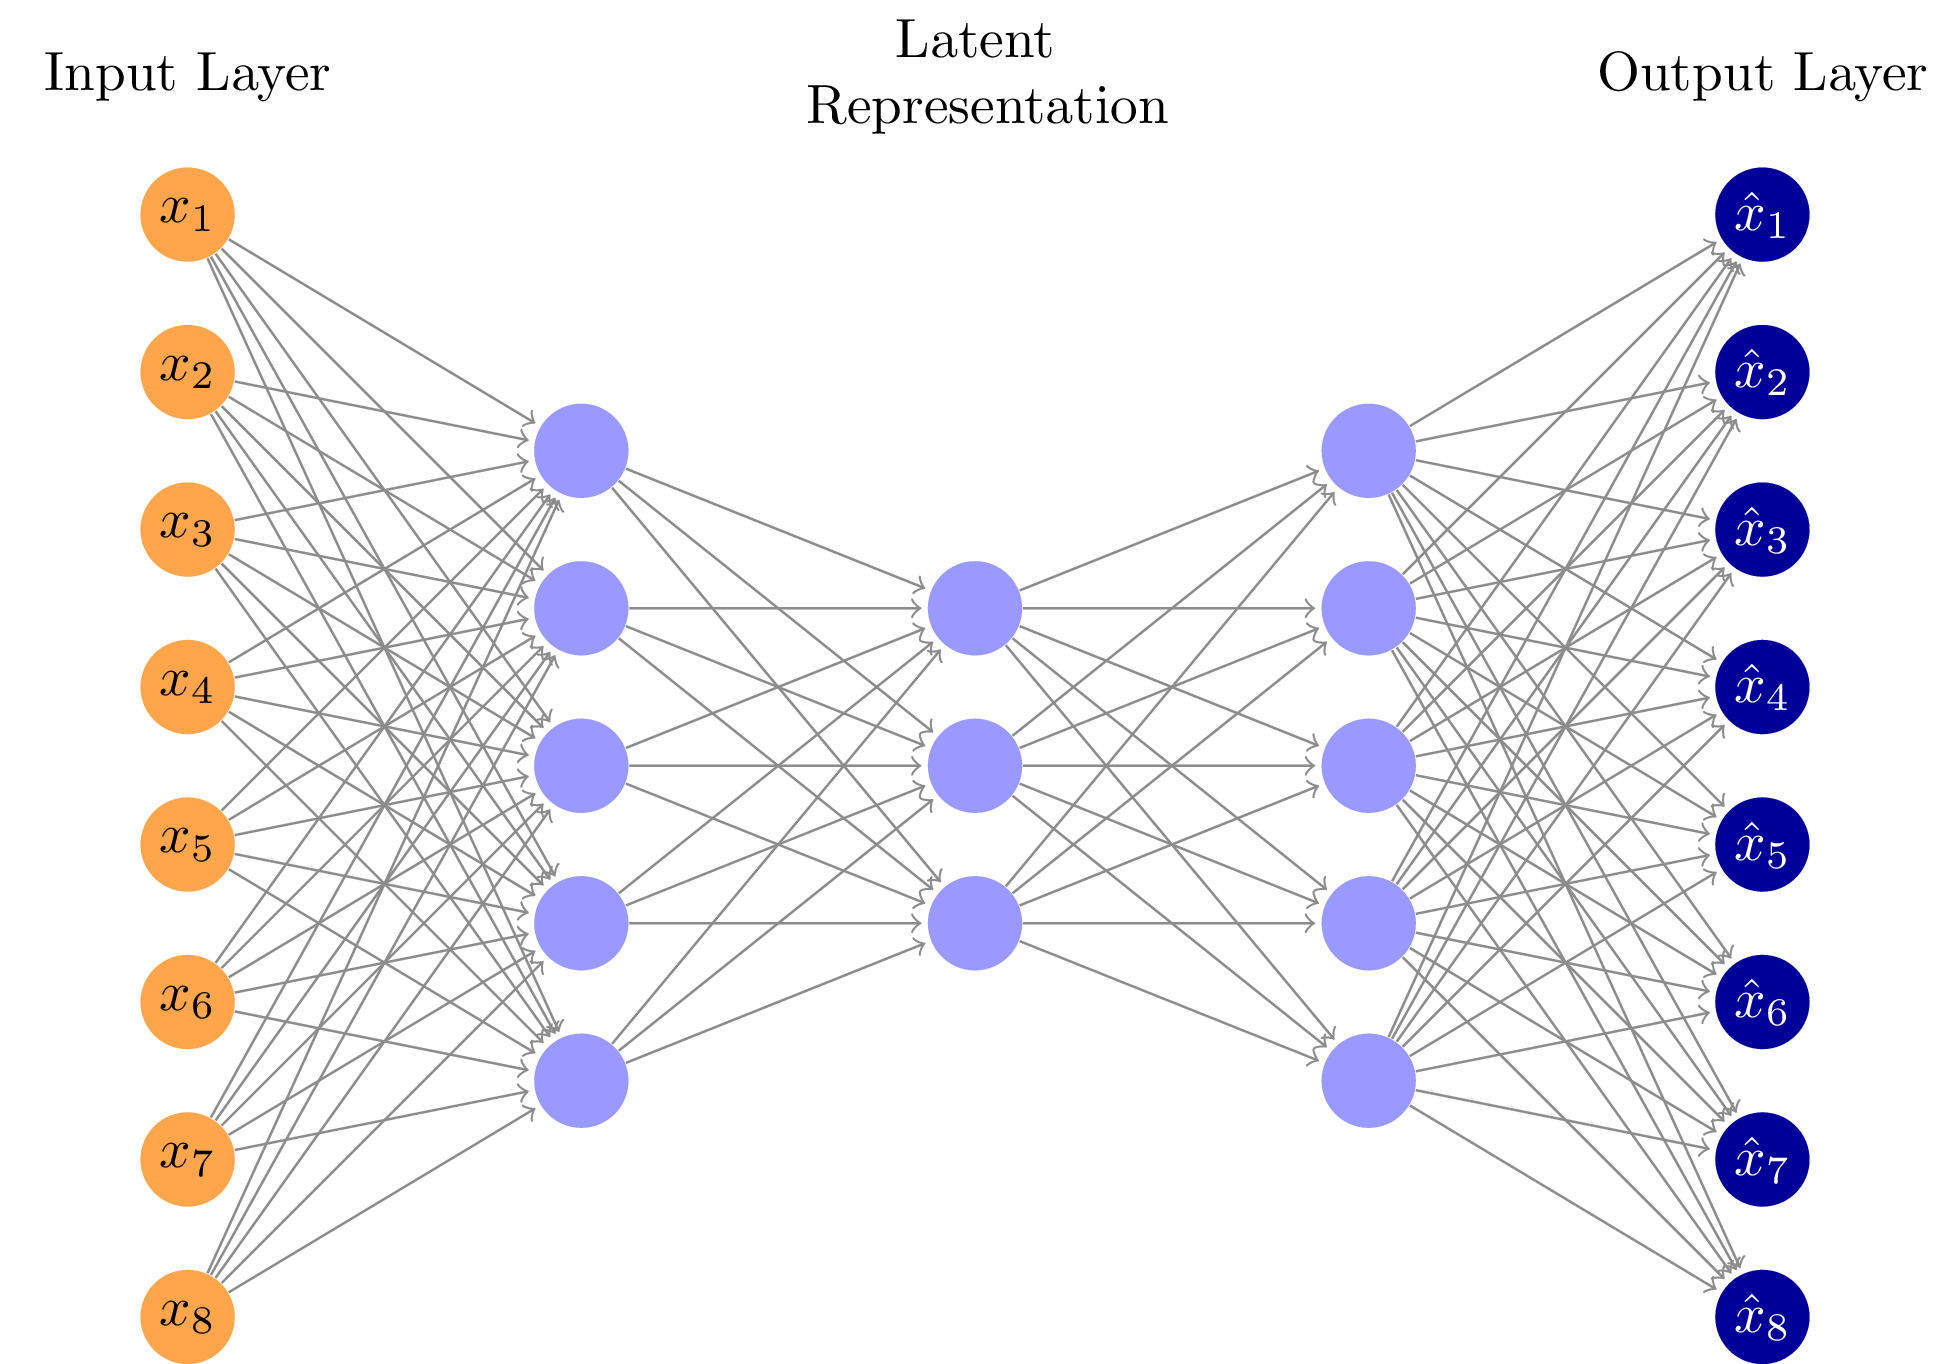
\includegraphics[width=\textwidth]{./../../Images/autoencoder_format.png}
		\end{figure}}
	\end{minipage}%
	\begin{minipage}[t]{0.4\textwidth}
	\begin{center}
		\begin{itemize}
			\item<4-> First Compression, then Decompression
			\item<5-> Input Dimension = Output Dimension
			\item<5-> Latent Dimension < Input Dimension
			\item<6-> Training: Minimize the MSE between Input and Output
			\item<7-> Compression Rate $CR = \frac{\text{Input Dimension}}{\text{Latent Dimension}}$
		\end{itemize}
	\end{center}
	\end{minipage}
	\begin{itemize}
		\item<8-> Different Network Architectures can have different CRs
		\item<8-> We're going to inspect CRs $2,4,8,16,32,64,128$
	\end{itemize}	
\end{frame}

\begin{frame}{Examples}
   \only<1>{ \begin{figure}
   		\centering
   		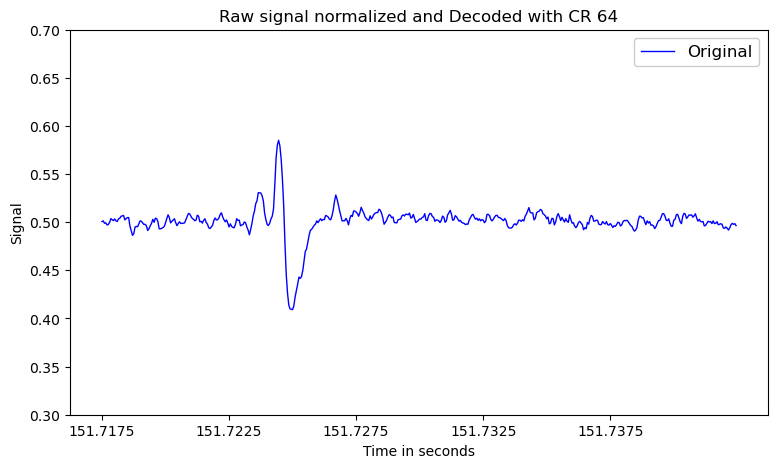
\includegraphics[width=\textwidth]{./../../Images/Presentation_Segment_Only.png}
   \end{figure}}
 \only<2>{ \begin{figure}
		\centering
		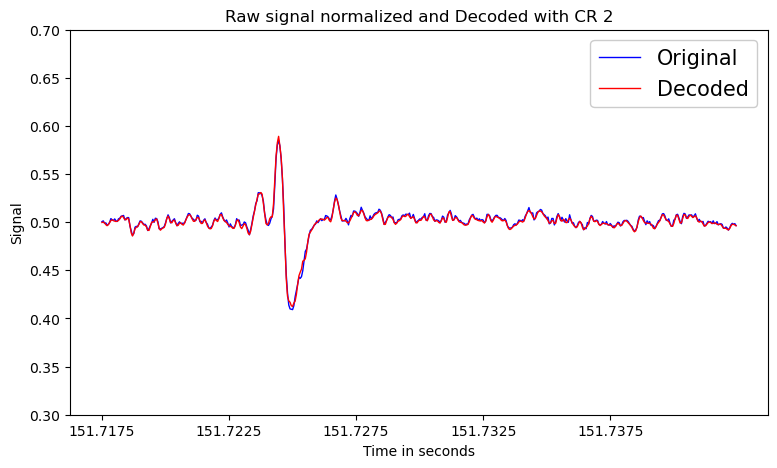
\includegraphics[width=\textwidth]{./../../Images/Presentation_Segment_CR2.png}
\end{figure}}
 \only<3->{ \begin{figure}
		\centering
		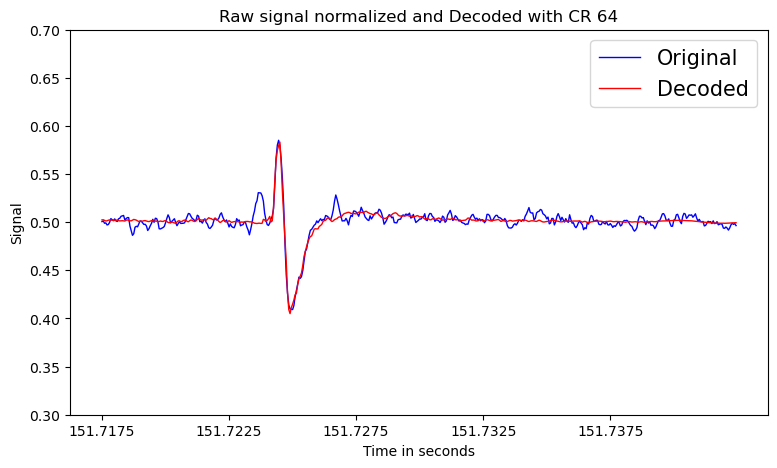
\includegraphics[width=\textwidth]{./../../Images/Presentation_Segment_CR64.png}
\end{figure}}
\only<3->{	\begin{itemize}
		\item<4> About 500 sample points
		\item<4> After compression only 8 points are stored!
\end{itemize}}
\end{frame}

\begin{frame}{Evaluation}
	\begin{figure}
			\centering
			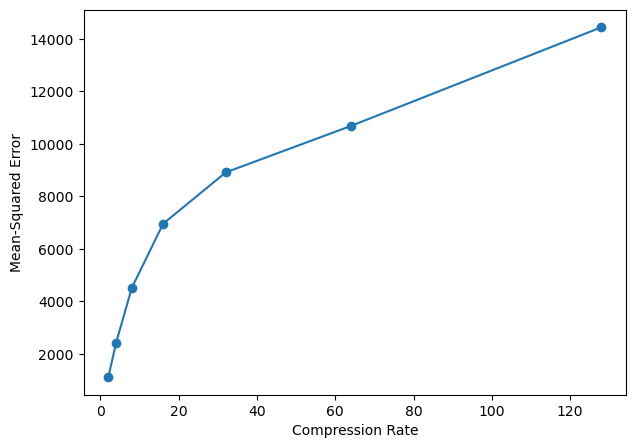
\includegraphics[height=0.9\textheight]{./../../Images/mse.png}
	\end{figure}
\end{frame}

\begin{frame}{Example continued}
	 \only<1>{ \begin{figure}
			\centering
			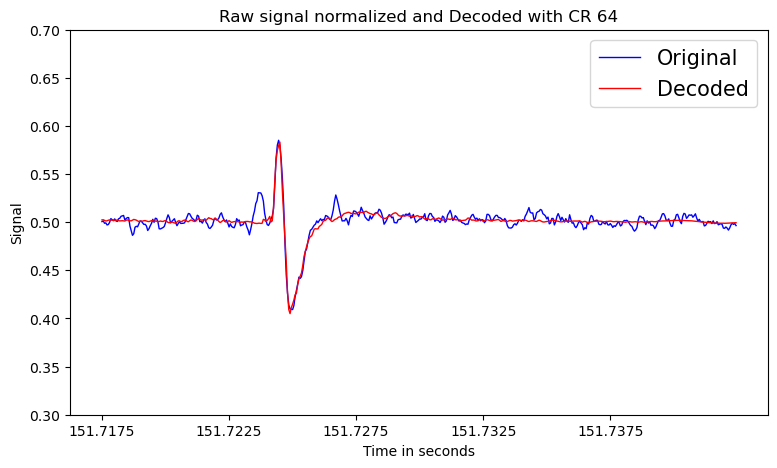
\includegraphics[width=\textwidth]{./../../Images/Presentation_Segment_CR64.png}
	\end{figure}}
	\only<1>{	\begin{itemize}
			\item<3> About 500 sample points
			\item<3> After compression only $\sim 8$ points are stored!
	\end{itemize}}
 \only<2>{ \begin{figure}
		\centering
		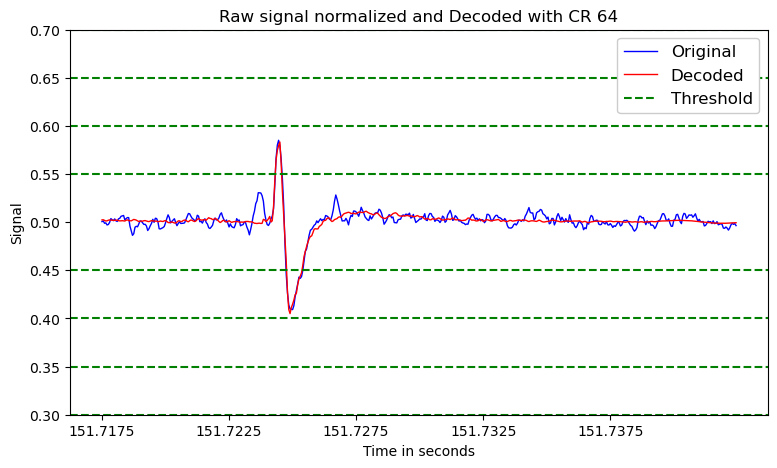
\includegraphics[width=\textwidth]{./../../Images/Presentation_Segment_CR64_all_thresholds.png}
\end{figure}}

 \only<3>{ \begin{figure}
		\centering
		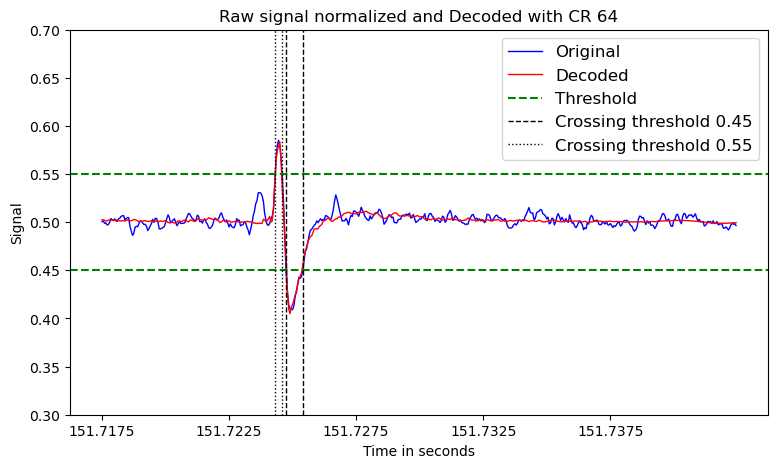
\includegraphics[width=\textwidth]{./../../Images/Presentation_Segment_CR64_thresholds_drawn.png}
	\end{figure}}

 \only<4->{ \begin{figure}
		\centering
		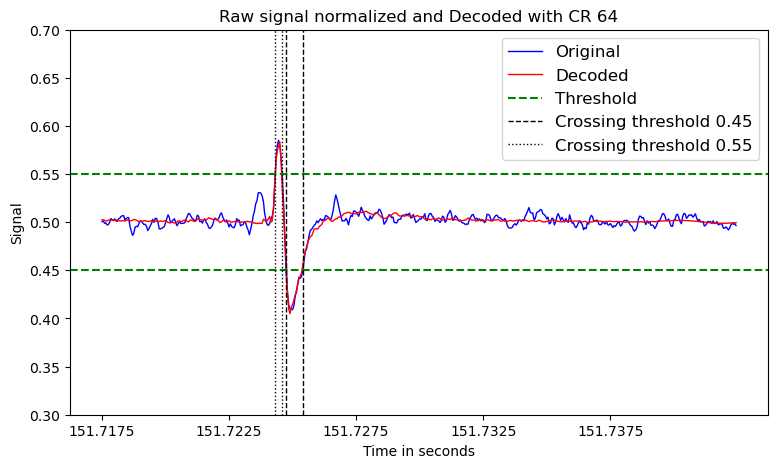
\includegraphics[width=0.7\textwidth]{./../../Images/Presentation_Segment_CR64_thresholds_drawn.png}
\end{figure}}
	\begin{itemize}
	\item<4-> How often does the original signal cross a threshold?
	\item<4-> How often does the decoded signal cross a threshold?
	\item<5-> How often does the original and the decoded signal cross a threshold at the exact same position? (preserved crossing)
	\end{itemize}
\end{frame}


\begin{frame}{Evaluation continued}
\only<1>{    \begin{minipage}[t]{0.5\textwidth}
		\begin{figure}
			\centering
			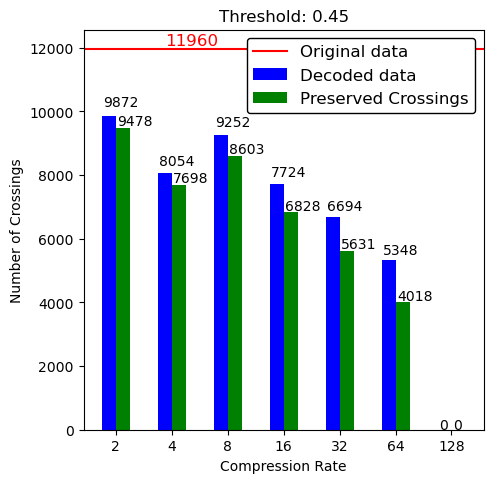
\includegraphics[width=\textwidth]{./../../Images/spikes_threshold_045.png}
		\end{figure}
	\end{minipage}%
	\begin{minipage}[t]{0.5\textwidth}
		\begin{figure}
			\centering
			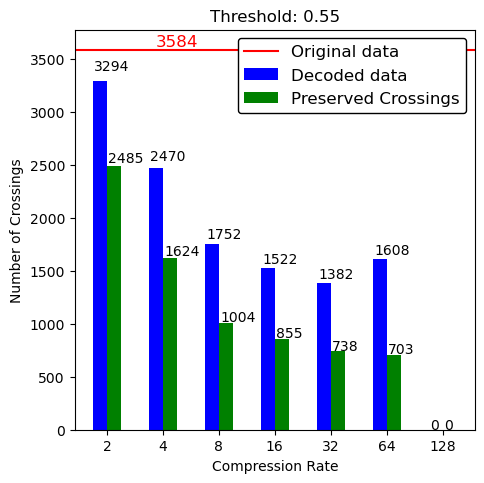
\includegraphics[width=\textwidth]{./../../Images/spikes_threshold_055.png}
		\end{figure}
\end{minipage}}
\only<2>{\begin{figure}
		\centering
		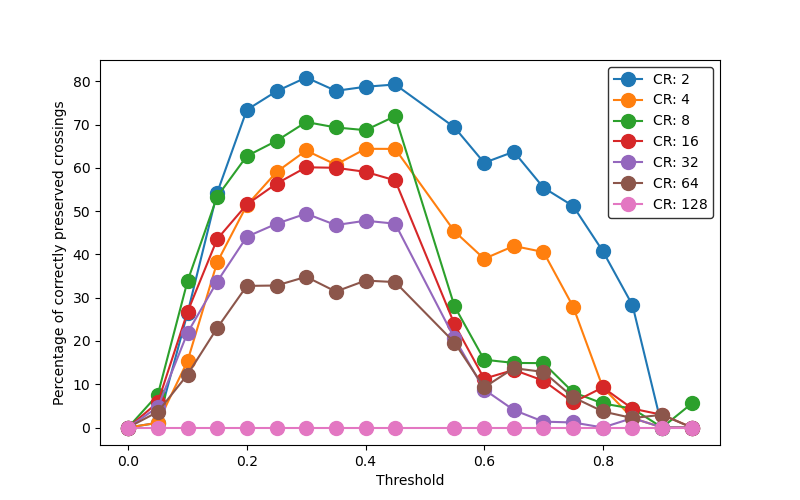
\includegraphics[height=0.9\textheight]{./../../Images/percentage_decoded.png}
\end{figure}}
\end{frame}

\begin{frame}{Conclusion}
	\begin{itemize}
		    \item<1-> Problems:  \begin{itemize}
		    	\item Identifying spikes
		    	\item Sorting spikes to individual nerve fibres
		    \end{itemize}
	     	\item<2-> Basic architecture of an autoencoder
	     	\item<3-> De-noising and smoothing of the signal 
	     	\item<4-> Performance differences for different compression rates

	\end{itemize}
\end{frame}

\begin{frame}{Future Work}
	\begin{itemize}
		\item<0-> Practical evaluation
		\item<1-> Optimize the autoencoder with more meaningful metric
		\item<2-> Check more auto-encoders, with smaller jumps in compression rate
	\end{itemize}
\end{frame}

\begin{frame}
    \begin{center}
        Thank you for listening!
    \end{center}
\end{frame}


\end{document}